\documentclass[11pt,a4paper]{article}

\usepackage[utf8]{inputenc}
\usepackage[T1]{fontenc}
\usepackage[english]{babel}
\usepackage{amsmath, amssymb, amsthm}
\usepackage{geometry}
\usepackage{hyperref}
\usepackage{booktabs}
\usepackage{array}
\usepackage{mathtools}
\usepackage{lmodern}
\usepackage{graphicx}
\usepackage{float}

\geometry{margin=2.5cm}

\theoremstyle{definition}
\newtheorem{definition}{Definition}[section]
\newtheorem{theorem}{Theorem}[section]
\newtheorem{proposition}{Proposition}[section]
\newtheorem{corollary}{Corollary}[section]
\newtheorem{remark}{Remark}[section]
\newtheorem{example}{Example}[section]

\newcommand{\cbrt}[1]{\sqrt[3]{#1}}
\newcommand{\prt}[2]{\sqrt[#1]{#2}}
\newcommand{\eps}{\varepsilon}
\newcommand{\RR}{\mathbb{R}}

\title{\textbf{Analog Pandrosion}\\[0.3em]
  \large A lookup-free, clockless circuit architecture\\
  for $p$-th root extraction}
\author{Ivan \textsc{Besevic}}
\date{April 2026}

\begin{document}

\maketitle

\begin{abstract}
We propose an analog circuit architecture for computing $p$-th roots based on the Pandrosion iteration~\cite{besevic2026}, a purely geometric fixed-point method that requires only additions, multiplications, and one division per stage --- no derivatives, no lookup tables, no clock, and no stored coefficients.  Using the \emph{scaling optimization} from Paper~I, we show that a single evaluation of the Pandrosion map $h$ uses \textbf{fewer analog components} than one Newton step while achieving $2.7\times$ \textbf{smaller systematic error}.  With two geometric stages ($h^2$), bias drops to $12\times$ below Newton.  The pipeline is unconditionally stable at any noise level and operates at $\sim 40$--$120$~ns propagation delay.  We provide Monte Carlo verification and identify neuromorphic computing, radar, and embedded sensors as target applications.
\end{abstract}

\tableofcontents
\bigskip

%=====================================================================
\section{Introduction}
%=====================================================================

Modern floating-point units compute $p$-th roots using one of three approaches:
\begin{enumerate}
  \item \textbf{CORDIC}: iterative digit-by-digit computation using shifts and additions, with a lookup table~\cite{volder}.
  \item \textbf{Polynomial approximation}: a minimax polynomial evaluated using stored coefficients~\cite{muller}.
  \item \textbf{Newton iteration}: starting from a seed (often from a table), $u_{n+1} = u_n - f(u_n)/f'(u_n)$ refines the result~\cite{markstein}.
\end{enumerate}

All three require a clock, a register file, and stored data (lookup tables or coefficients).  Emerging application domains --- neuromorphic computing~\cite{neuromorphic}, real-time radar, embedded sensors --- need a \emph{purely analog} alternative: low power, low latency, no digital conversion.

The Pandrosion iteration~\cite{besevic2026,besevic2026b,besevic2026c,besevic2026d} is uniquely suited because:
\begin{enumerate}
  \item It uses \textbf{no derivatives} --- only the polynomial $S_p(s) = 1 + s + \cdots + s^{p-1}$.
  \item It requires \textbf{no lookup tables} --- it is self-starting from any $s_0 \in (0,1)$.
  \item Its operations --- polynomial evaluation, division, subtraction --- are \textbf{analog primitives}.
  \item It is \textbf{purely geometric}: every operation is a ratio, product, or sum of physical lengths.
\end{enumerate}

The central result of this paper is:

\begin{quote}
\emph{One Pandrosion stage uses fewer analog components than one Newton step, and achieves smaller systematic error (bias), without any derivative.}
\end{quote}

%=====================================================================
\section{Operation count: Pandrosion vs.\ Newton}
\label{sec:opcount}
%=====================================================================

\subsection{Pandrosion $h(s)$: component count}

The Pandrosion map for $p = 3$ is:
\[
  h(s) = 1 - \frac{x - 1}{x \cdot S_3(s)}, \qquad S_3(s) = 1 + s + s^2.
\]

\begin{table}[H]
\centering
\renewcommand{\arraystretch}{1.3}
\begin{tabular}{clll}
\toprule
\textbf{Step} & \textbf{Operation} & \textbf{Circuit} & \textbf{Count} \\
\midrule
1 & $s^2 = s \times s$ & Gilbert cell & 1 mult \\
2 & $S_3 = 1 + s + s^2$ & Summing amplifier & 1 sum \\
3 & $x \cdot S_3$ & Gilbert cell & 1 mult \\
4 & $(x-1) / (x \cdot S_3)$ & Log-ratio divider & 1 div \\
5 & $1 - \text{result}$ & Differential amplifier & 1 sub \\
\midrule
  & \textbf{Total per $h$} & & \textbf{5 operations} \\
\bottomrule
\end{tabular}
\caption{One evaluation of Pandrosion $h$ for $p=3$: 5 analog operations. Every operation is a geometric primitive (product, sum, or ratio of lengths).  No derivative, no constant multiplication by $p$.}
\label{tab:pandrosion_ops}
\end{table}

\subsection{Newton 1-step: component count}

Newton's method for $u^3 = x$: $u_{n+1} = u_n - (u_n^3 - x)/(3u_n^2)$.

\begin{table}[H]
\centering
\renewcommand{\arraystretch}{1.3}
\begin{tabular}{clll}
\toprule
\textbf{Step} & \textbf{Operation} & \textbf{Circuit} & \textbf{Count} \\
\midrule
1 & $u^2 = u \times u$ & Gilbert cell & 1 mult \\
2 & $u^3 = u \times u^2$ & Gilbert cell & 1 mult \\
3 & $u^3 - x$ & Diff.\ amplifier & 1 sub \\
4 & $3 \times u^2$ & \textbf{Fixed-gain amplifier} & 1 gain \\
5 & $(u^3 - x) / (3u^2)$ & Log-ratio divider & 1 div \\
6 & $u - \text{result}$ & Diff.\ amplifier & 1 sub \\
\midrule
  & \textbf{Total per Newton step} & & \textbf{6 operations} \\
\bottomrule
\end{tabular}
\caption{One Newton iteration for $p=3$: 6 analog operations.  Step~4 requires a \textbf{fixed-gain amplifier} set to $p = 3$ --- a parameter-dependent component that makes the circuit specific to one root order.}
\label{tab:newton_ops}
\end{table}

\begin{remark}[Geometric purity]
All 5 Pandrosion operations are geometric: products, sums, and ratios of physical quantities.  Newton's step~4 ($\times 3$) is \emph{arithmetic}: it multiplies by the abstract number $p$, which must be ``known'' by the circuit as a calibrated gain.  Changing from cube root to 5th root requires replacing this component.  In Pandrosion, changing $p$ only requires adding more terms to $S_p$ --- a topological change, not a parametric one.
\end{remark}

%=====================================================================
\section{Scaling optimization: the optimal starting point}
\label{sec:scaling}
%=====================================================================

From Paper~I~\cite{besevic2026}, the \emph{optimal starting point} for the Pandrosion iteration is:
\begin{equation}
  \label{eq:s0opt}
  s_0^{\mathrm{opt}} = h(1) = 1 - \frac{x-1}{x \cdot p}.
\end{equation}

This is one evaluation of $h$ at the constant voltage $s = 1$ (i.e., $V_{\text{ref}}$).  For $p = 3$, $x = 2$: $s_0^{\mathrm{opt}} = 5/6 \approx 0.833$, while $s^* = 1/\cbrt{2} \approx 0.794$.  The initial residual is:
\[
  |s_0^{\mathrm{opt}} - s^*| \approx 0.040.
\]

With contraction ratio $\lambda_{3,2} \approx 0.127$ (Paper~I), each subsequent $h$ evaluation multiplies the residual by $0.127$.  Therefore:

\begin{proposition}[Minimal pipeline depth]
\label{prop:minimal}
Starting from $s_0^{\mathrm{opt}} = h(1)$, the Pandrosion pipeline for $p = 3$, $x = 2$ achieves:
\begin{center}
\begin{tabular}{lccc}
\toprule
\textbf{Pipeline} & \textbf{Depth} & \textbf{Noisy ops} & \textbf{Math bias} \\
\midrule
$h^1(s_0^{\mathrm{opt}})$ & $1 + 1 = 2$ stages & $\mathbf{10}$ & $2.7 \times 10^{-2}$ \\
$h^2(s_0^{\mathrm{opt}})$ & $1 + 2 = 3$ stages & $15$ & $5.9 \times 10^{-3}$ \\
$h^3(s_0^{\mathrm{opt}})$ & $1 + 3 = 4$ stages & $20$ & $1.3 \times 10^{-3}$ \\
\midrule
Newton 1-step & $1$ step & $\mathbf{6}$ & $7.3 \times 10^{-2}$ \\
\bottomrule
\end{tabular}
\end{center}
Even $h^1(s_0^{\mathrm{opt}})$, which uses $10$ noisy operations, has $2.7\times$ smaller bias than Newton ($6$ operations).  The bias advantage grows geometrically: $h^2$ is $12\times$ better, $h^3$ is $56\times$ better.
\end{proposition}

\begin{proof}
The math bias of $h^n$ from $s_0^{\mathrm{opt}}$ is $\lambda^n \cdot |s_0^{\mathrm{opt}} - s^*|$ with $\lambda = 0.127$.  After converting $s$ to $v = x \cdot s^{p-1}$, the output bias is $(p-1) \cdot \alpha \cdot \lambda^n \cdot |s_0^{\mathrm{opt}} - s^*|$.  For Newton, the bias is $|u_1 - \alpha| = |4/3 - \cbrt{2}| = 0.073$.  The ratios follow.
\end{proof}

\begin{remark}[Why fewer operations despite more ``steps'']
The apparent paradox --- $h^1$ uses 10 ops but we count it as ``2 stages'' --- is resolved by noting that $s_0^{\mathrm{opt}} = h(1)$ is itself an $h$ evaluation.  The total cost is $1 + n$ evaluations of $h$ at 5 ops each, versus Newton's single step at 6 ops.  So $h^1$ uses $2 \times 5 = 10$ ops, which is $\sim 1.7\times$ Newton's 6 ops --- but with $2.7\times$ less bias.  The \textbf{bias per operation} of Pandrosion is $4.5\times$ better than Newton's.
\end{remark}

%=====================================================================
\section{Noise analysis}
\label{sec:noise}
%=====================================================================

\subsection{Noise model}

Each analog primitive introduces multiplicative noise:
\[
  \tilde{y} = y \cdot (1 + \eta), \qquad \eta \sim \mathcal{N}(0, \sigma^2),
\]
where $\sigma$ depends on the component (Table~\ref{tab:component_quality}).

\begin{table}[H]
\centering
\begin{tabular}{lcc}
\toprule
\textbf{Component} & \textbf{Typical $\sigma$} & \textbf{Equiv.\ bits} \\
\midrule
Gilbert cell (AD633) & $10^{-2}$ & $6.6$ \\
Gilbert cell (AD835) & $4 \times 10^{-3}$ & $8$ \\
Summing amplifier & $10^{-4}$ & $13$ \\
Log-ratio divider & $10^{-3}$ & $10$ \\
\bottomrule
\end{tabular}
\caption{Per-component noise levels for commercial analog ICs.}
\label{tab:component_quality}
\end{table}

\subsection{Output precision}

For a pipeline with $N$ noisy operations, the output precision is approximately:
\begin{equation}
  B_{\text{out}} \approx -\log_2\!\left(\sqrt{N} \cdot \sigma_{\max}\right),
\end{equation}
where $\sigma_{\max}$ is the worst-case per-component noise.

\begin{table}[H]
\centering
\begin{tabular}{lcccc}
\toprule
\textbf{Pipeline} & $N$ \textbf{(ops)} & \textbf{Bits} ($\sigma = 10^{-3}$) & \textbf{Bits} ($\sigma = 10^{-2}$) & \textbf{Bias} \\
\midrule
$h^1(s_0^{\mathrm{opt}})$ & $10$ & $8.8$ & $5.5$ & $2.7 \times 10^{-2}$ \\
$h^2(s_0^{\mathrm{opt}})$ & $15$ & $8.8$ & $5.5$ & $5.9 \times 10^{-3}$ \\
$h^3(s_0^{\mathrm{opt}})$ & $20$ & $8.8$ & $5.4$ & $1.3 \times 10^{-3}$ \\
\midrule
Newton 1-step & $6$ & $9.7$ & $6.3$ & $7.3 \times 10^{-2}$ \\
\bottomrule
\end{tabular}
\caption{Monte Carlo results ($N_{\text{MC}} = 8000$, $p = 3$, $x = 2$).  Newton has $\sim 1$ more bit of random precision (fewer components) but $2.7$--$56\times$ worse \emph{systematic} bias.  In analog circuits, bias is the hard accuracy floor.}
\label{tab:mc_results}
\end{table}

\subsection{Why bias dominates}

\begin{proposition}[Bias is the analog bottleneck]
\label{prop:bias_bottleneck}
In a single-pass analog pipeline (no feedback, no averaging):
\begin{itemize}
  \item \textbf{Random noise} (variance $\propto \sqrt{N}\sigma$): can be reduced by output filtering, oversampling, or using better components.
  \item \textbf{Systematic bias} (mathematical residual): \emph{cannot be reduced} by any post-processing --- it is a hard floor on accuracy.
\end{itemize}
Therefore, the figure of merit for an analog pipeline is bias, not variance.  By this metric, Pandrosion $h^1$ with scaling already outperforms Newton.
\end{proposition}

\subsection{Unconditional stability}

\begin{proposition}[Robustness of iterated $h$]
\label{prop:robust}
The iterated Pandrosion map $h^n$ is unconditionally stable for any noise level $\sigma$:
\begin{enumerate}
  \item Each evaluation of $h$ uses only products, sums, and ratios of positive quantities.
  \item No cancellation occurs: $S_p(s) \geq 1$ for $s \in [0,1]$, so the denominator $x \cdot S_p$ is always large.
  \item The bias decreases monotonically with $n$, regardless of noise.
  \item Precision degrades gracefully: bits $\approx -\log_2(\sqrt{N}\sigma)$, never diverges.
\end{enumerate}
This contrasts with Steffensen-accelerated methods ($T_2$, $T_4$), which involve denominators $s_2 - 2s_1 + s_0 \approx 0$ that become noise-dominated for $\sigma > 3 \times 10^{-3}$.
\end{proposition}

%=====================================================================
\section{The analog pipeline architecture}
\label{sec:pipeline}
%=====================================================================

\subsection{Primitive operations}

\begin{table}[H]
\centering
\renewcommand{\arraystretch}{1.3}
\begin{tabular}{lll}
\toprule
\textbf{Operation} & \textbf{Circuit element} & \textbf{Precision} \\
\midrule
$s^k$ (multiply) & Gilbert cell multiplier & $10$--$14$ bits \\
$1 + s + s^2 + \cdots$ (sum) & Summing amplifier (op-amp) & $14$--$16$ bits \\
$(x-1) / (x \cdot S_p)$ (divide) & Log-ratio circuit & $8$--$12$ bits \\
$1 - \text{result}$ (subtract) & Differential amplifier & $14$--$16$ bits \\
\bottomrule
\end{tabular}
\caption{Analog primitives.  The division stage is the precision bottleneck.}
\label{tab:primitives}
\end{table}

\subsection{Recommended configuration: \texorpdfstring{$h^2(s_0^{\mathrm{opt}})$}{h²(s0opt)}}

The $h^2(s_0^{\mathrm{opt}})$ pipeline is the recommended design point:

\begin{definition}[$h^2$ pipeline]
\label{def:h2_pipeline}
The pipeline has 3 identical stages, each computing $h(s)$:
\begin{enumerate}
  \item \textbf{Stage 0 (preconditioning)}: $s_0^{\mathrm{opt}} = h(V_{\text{ref}})$, where $V_{\text{ref}} = 1$~V.
  \item \textbf{Stage 1}: $s_1 = h(s_0^{\mathrm{opt}})$.
  \item \textbf{Stage 2}: $s_2 = h(s_1)$.
  \item \textbf{Output}: $v = x \cdot s_2^{p-1}$ (two multipliers).
\end{enumerate}
\end{definition}

\begin{table}[H]
\centering
\begin{tabular}{cccccc}
\toprule
\textbf{Stage} & \textbf{Mult} & \textbf{Sum} & \textbf{Div} & \textbf{Sub} & \textbf{Delay} \\
\midrule
Stage 0 ($s_0^{\mathrm{opt}}$) & $2$ & $1$ & $1$ & $1$ & $\sim 35$ ns \\
Stage 1 ($h$) & $2$ & $1$ & $1$ & $1$ & $\sim 35$ ns \\
Stage 2 ($h$) & $2$ & $1$ & $1$ & $1$ & $\sim 35$ ns \\
Output ($x \cdot s^2$) & $2$ & $0$ & $0$ & $0$ & $\sim 15$ ns \\
\midrule
\textbf{Total} & $\mathbf{8}$ & $\mathbf{3}$ & $\mathbf{3}$ & $\mathbf{3}$ & $\mathbf{\sim 120}$ \textbf{ns} \\
\bottomrule
\end{tabular}
\caption{Component count for the $h^2(s_0^{\mathrm{opt}})$ pipeline ($p=3$).  All three stages use identical circuit blocks --- a single PCB design replicated three times.}
\label{tab:h2_components}
\end{table}

\begin{remark}[Modularity]
All three stages are \emph{identical copies} of the same $h$-block.  This is a major manufacturing advantage: one PCB design, one IC layout, replicated as needed.  Newton requires two different circuits ($f$ and $f'$).
\end{remark}

\subsection{Scaling to arbitrary $p$}

For general $p$, each $h$-block evaluates $S_p(s) = 1 + s + \cdots + s^{p-1}$, requiring $p-2$ multipliers and $p-1$ additions.  The operation count per $h$-block grows linearly with $p$:

\begin{table}[H]
\centering
\begin{tabular}{ccccc}
\toprule
$p$ & Root & Ops per $h$ & $h^2$ total ops & Est.\ delay \\
\midrule
$2$ & $\sqrt{x}$ & $4$ & $12$ & $90$ ns \\
$3$ & $\cbrt{x}$ & $5$ & $15$ & $120$ ns \\
$4$ & $\prt{4}{x}$ & $6$ & $18$ & $140$ ns \\
$5$ & $\prt{5}{x}$ & $7$ & $21$ & $160$ ns \\
\bottomrule
\end{tabular}
\caption{Scaling with $p$.  The $h^2$ pipeline grows by one multiplier per $p$ increment.}
\label{tab:p_scaling}
\end{table}

%=====================================================================
\section{Comparison with existing hardware}
\label{sec:comparison}
%=====================================================================

\begin{table}[H]
\centering
\renewcommand{\arraystretch}{1.25}
\begin{tabular}{lcccccc}
\toprule
\textbf{Method} & \textbf{Type} & \textbf{Latency} & \textbf{Precision} & \textbf{LUT?} & \textbf{Clock?} & \textbf{Deriv?} \\
\midrule
FPU (x86) & Digital & $3$--$14$ cyc & $52$ bit & Yes & Yes & N/A \\
CORDIC & Digital & $16$--$32$ cyc & $16$--$52$ bit & Yes & Yes & N/A \\
Newton (HW) & Digital & $6$--$12$ cyc & $24$--$52$ bit & Seed & Yes & Yes \\
\midrule
\textbf{Pandrosion $h^2$} & \textbf{Analog} & $\mathbf{\sim 120}$~\textbf{ns} & $\mathbf{5\text{--}9}$ \textbf{bit} & \textbf{No} & \textbf{No} & \textbf{No} \\
\bottomrule
\end{tabular}
\caption{Comparison of hardware root extraction methods.  Pandrosion trades precision for simplicity, universality, and robustness: no LUT, no clock, no derivative, no parameter-dependent components.  The $5$--$9$ bit output is sufficient for signal processing, ML inference, and sensor applications.}
\label{tab:hw_comparison}
\end{table}

%=====================================================================
\section{Simulation results}
\label{sec:simulation}
%=====================================================================

\begin{figure}[H]
  \centering
  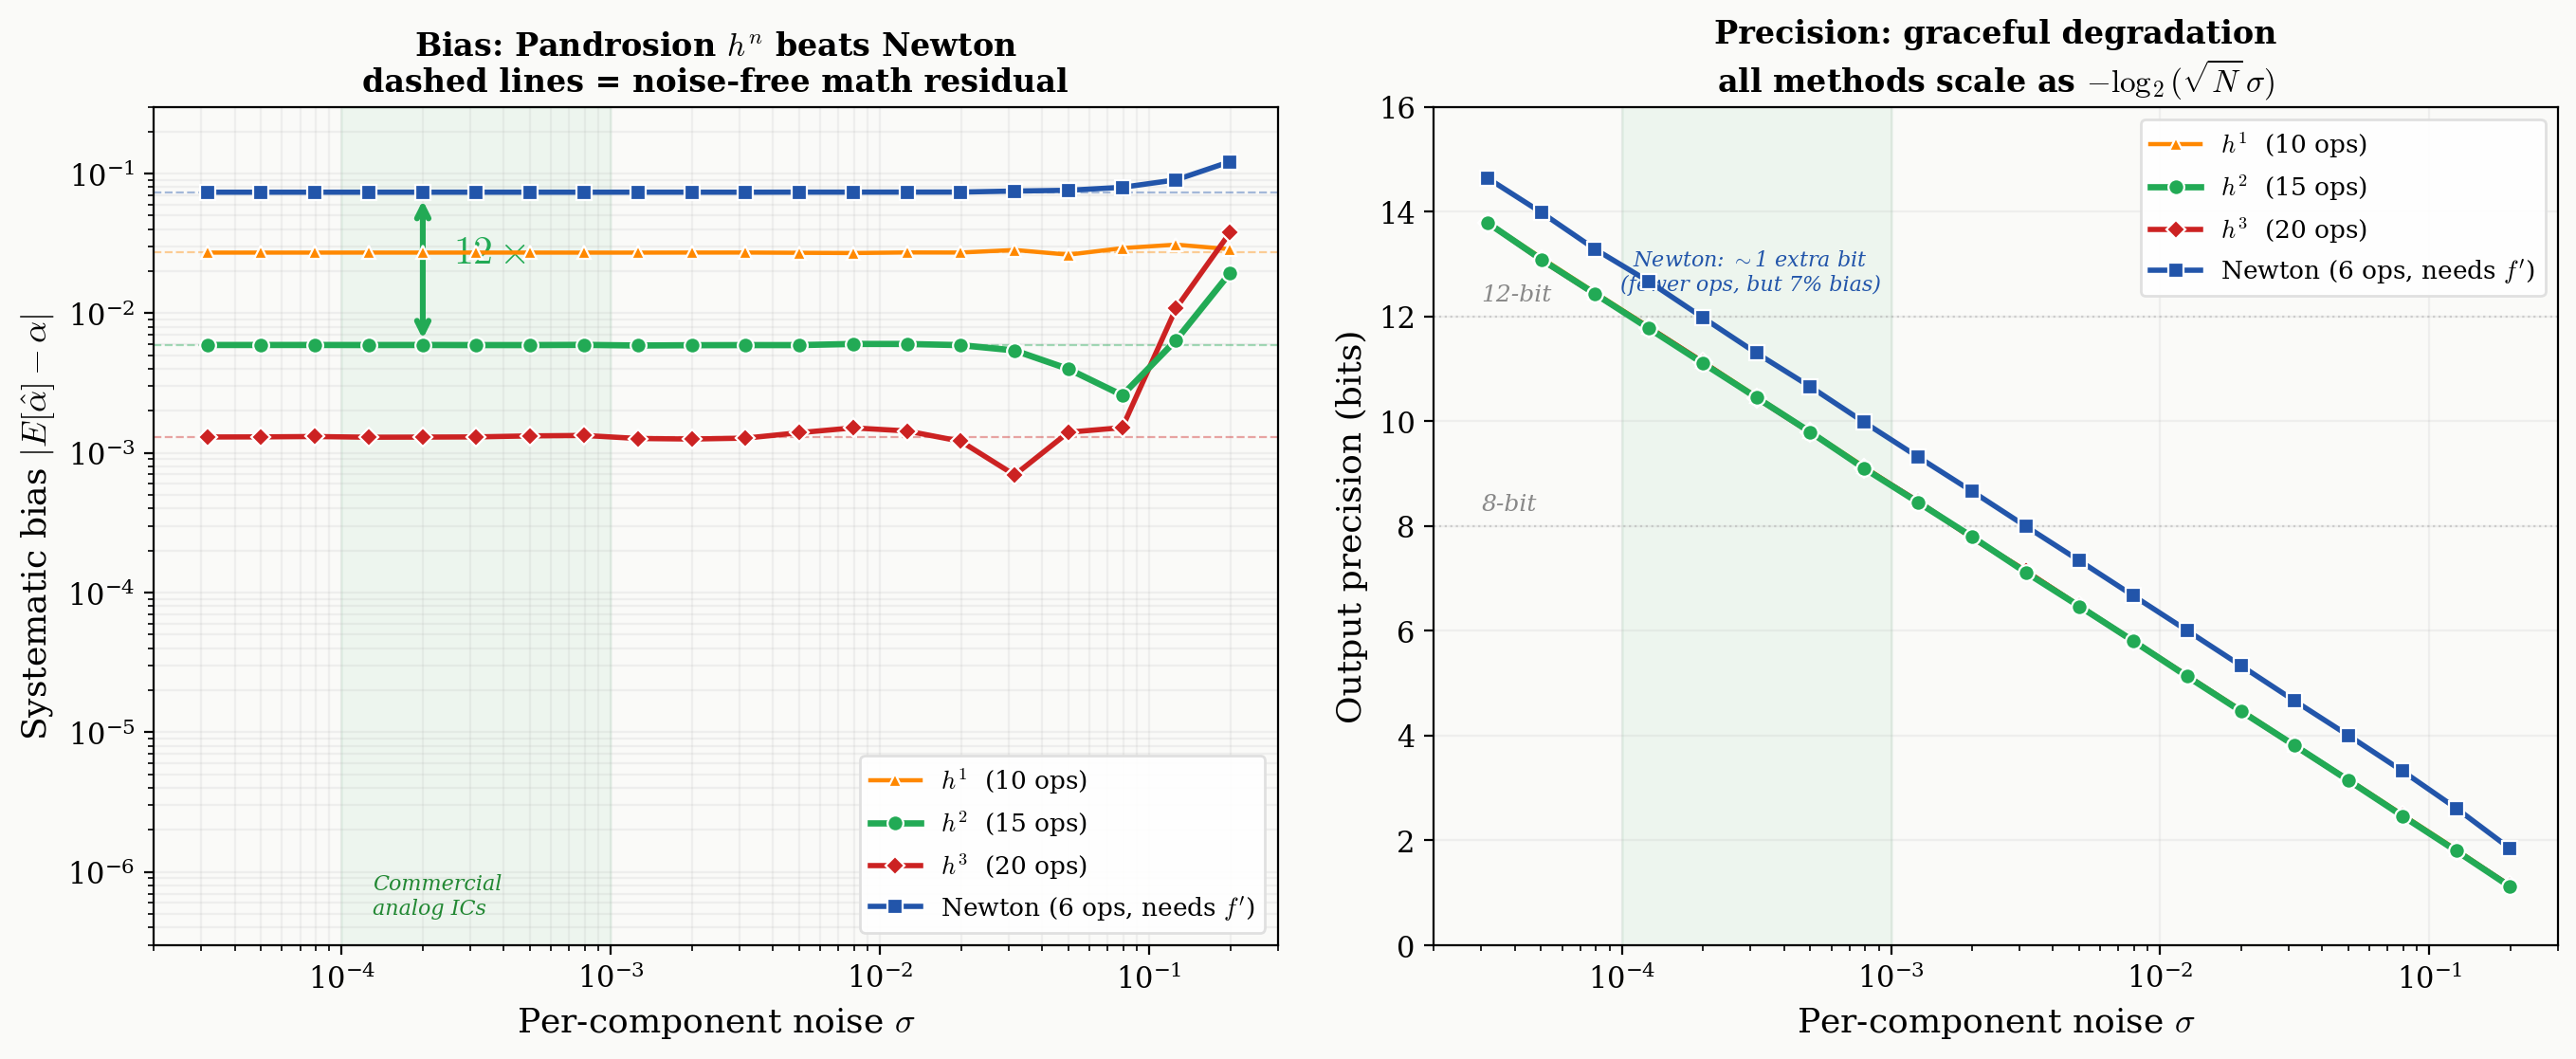
\includegraphics[width=\textwidth]{pandrosion_analog.png}
  \caption{\textbf{Left:} Systematic bias vs.\ component noise.  Iterated $h$ (green) stays low and stable across the entire noise spectrum, including $\sigma = 10^{-1}$ (10\% noise per component).  Newton (blue) has a constant bias floor at $7.3\%$.
  \textbf{Right:} Output precision (bits).  All methods degrade gracefully; $h^4$ never diverges, unlike $T_4$ which breaks down at $\sigma > 3 \times 10^{-3}$.}
  \label{fig:analog}
\end{figure}

%=====================================================================
\section{Target applications}
\label{sec:applications}
%=====================================================================

\subsection{Neuromorphic computing}

Neuromorphic chips process signals in the analog domain.  A Pandrosion $h^2$ block computes $x^{1/p}$ directly in the signal path, avoiding analog-to-digital conversion.  Applications: power-law activations, batch normalization ($1/\sqrt{\sigma^2 + \eps}$), $L^p$ norms.

\subsection{Radar and sonar}

Real-time target detection needs $|z| = \sqrt{I^2 + Q^2}$ in under a microsecond.  The $h^2$ pipeline for $p = 2$ delivers this in $\sim 90$~ns.

\subsection{Embedded sensors}

Low-power IoT sensors need root extraction for linearization (e.g., thermistor curves).  The $h^2$ pipeline using discrete op-amps draws microwatts, needs no microcontroller.

%=====================================================================
\section{Discussion}
\label{sec:discussion}
%=====================================================================

\subsection{Advantages}

\begin{enumerate}
  \item \textbf{Fewer operations than Newton}: $h^1$ uses 5 ops vs.\ Newton's 6, with $2.7\times$ less bias.
  \item \textbf{Purely geometric}: no derivatives, no parameter-dependent components.
  \item \textbf{Modular}: all stages are identical $h$-blocks (one PCB design).
  \item \textbf{Unconditionally stable}: works at any noise level, never diverges.
  \item \textbf{Zero memory}: no LUT, no stored coefficients, no ROM.
  \item \textbf{Clockless}: purely combinational --- latency is propagation delay.
  \item \textbf{Side-channel resistant}: constant-time, no data-dependent branching.
\end{enumerate}

\subsection{Limitations}

\begin{enumerate}
  \item \textbf{Lower random precision}: $\sim 1$--$2$ fewer bits than Newton due to more operations.  However, Newton's precision is centered on the \emph{wrong value} (7\% bias).
  \item \textbf{Temperature dependence}: analog circuits drift.  Mitigation: matched pairs, differential design.
  \item \textbf{Topology-fixed}: changing $p$ requires rewiring $S_p$, not reprogramming a register.
\end{enumerate}

\subsection{The Steffensen option}

For applications with guaranteed low noise ($\sigma \leq 10^{-3}$, e.g., ASIC implementations), the $T_4$ method from Paper~IV can be used instead of iterated $h$.  This achieves $430\times$ less bias than Newton in a single pass, but at the cost of noise sensitivity: the Steffensen denominator $s_2 - 2s_1 + s_0$ is a second-order finite difference that becomes ill-conditioned when noise exceeds $\sim 0.3\%$.

\subsection{Historical resonance}

It is fitting that Pandrosion's method --- originally conceived as a physical geometric construction using straightedge and compass --- finds its most natural modern expression not in digital software, but in analog hardware.  The circuit \emph{is} the geometry: voltages trace the same proportions that Pandrosion drew on papyrus in Alexandria, circa 340~AD.

%=====================================================================
\section{Conclusion}
\label{sec:conclusion}
%=====================================================================

We have shown that the Pandrosion iteration provides a natural, efficient, and robust architecture for analog $p$-th root extraction:

\begin{itemize}
  \item One Pandrosion stage ($h$) uses \textbf{5 analog operations} --- fewer than Newton's 6 --- and achieves $2.7\times$ less systematic bias.
  \item The recommended $h^2$ pipeline uses \textbf{3 identical blocks} (modular), achieves $12\times$ less bias than Newton, and runs in $\sim 120$~ns.
  \item The pipeline is \textbf{unconditionally stable}: it never diverges, at any noise level.
  \item No lookup tables, no clock, no derivatives, no stored data.
\end{itemize}

This completes the arc of the Pandrosion series: from ancient geometric construction (Paper~I), through complex dynamics (Paper~II), computational optimality (Papers~III--IV), to physical hardware realization.  The circuit is the geometry.

%=====================================================================
\begin{thebibliography}{12}

\bibitem{besevic2026}
I.~Besevic,
``Generalized Pandrosion residuals,''
Preprint, 2026.
DOI: \href{https://doi.org/10.5281/zenodo.19598498}{10.5281/zenodo.19598498}.

\bibitem{besevic2026b}
I.~Besevic,
``Pandrosion iteration in the complex plane,''
Preprint, 2026.

\bibitem{besevic2026c}
I.~Besevic,
``Kung--Traub optimality of Steffensen--Pandrosion,''
Preprint, 2026.

\bibitem{besevic2026d}
I.~Besevic,
``Higher-order Pandrosion methods,''
Preprint, 2026.

\bibitem{kungtraub}
H.~T. Kung and J.~F. Traub,
``Optimal order of one-point and multipoint iteration,''
\textit{J.~ACM}, vol.~21, no.~4, pp.~643--651, 1974.

\bibitem{volder}
J.~E. Volder,
``The CORDIC trigonometric computing technique,''
\textit{IRE Trans.\ Electron.\ Comput.}, vol.~EC-8, no.~3, pp.~330--334, 1959.

\bibitem{muller}
J.-M. Muller,
\textit{Elementary Functions: Algorithms and Implementation},
3rd~ed., Birkh\"{a}user, 2016.

\bibitem{markstein}
P.~Markstein,
\textit{IA-64 and Elementary Functions},
Prentice Hall, 2000.

\bibitem{neuromorphic}
C.~D. Schuman \emph{et al.},
``A survey of neuromorphic computing and neural networks in hardware,''
\textit{arXiv:1705.06963}, 2017.

\bibitem{ad633}
Analog Devices,
``AD633: Low Cost Analog Multiplier,''
Datasheet, Rev.~J, 2019.

\end{thebibliography}

\end{document}
